\documentclass[10pt]{article}
\usepackage{icmlko}

\icmlmeta{IP 파운데이션 월드모델}{207}{분모가 바뀌었지 세계가 바뀐 게 아니다}{노트 182부터 스물다섯 노트가 웹툰의 부호 역전을 ``시간에 시든다''로 다뤘다. 축의 정의를 열어 보니 분모에 긁은 날이 박혀 있었다}

\begin{document}

\twocolumn[
\icmlheader

\begin{abstract}
노트 206이 ``웹툰 \texttt{goods\_scale} 이 왜 2022년에 뒤집혔나''를 남기고
연재 정책 변화를 후보로 걸었다. 축의 정의부터 봤다 --- 축 파일의
\texttt{why} 가 ``연재 밀도 258화/299주''다. \textbf{회차 수 $\div$ 시작
이후 경과 주}이고, 그 ``이후''의 끝이 \emph{긁은 날}로 고정돼 있다.
\textbf{그래서 최근 작품일수록 분모가 작다} --- 시작 연도별 경과 주 중앙이
2018년 \textbf{418주}에서 2026년 \textbf{8주}로 무너지고, 밀도 중앙이
0.367 에서 \textbf{2.685} 로 폭발한다. 완결율도 94.4\%에서 20.7\%로 떨어져
분자마저 잘려 있다. \textbf{그러니 이 축이 재는 것은 연재 밀도가 아니라
``얼마나 최근에 시작했나''다.} 검정했다 --- 경과 주를 통제하면 유보 상관이
\textbf{$-$0.312 에서 $-$0.031} 로 사라지고, 학습은 $+$0.378 에서 $+$0.562
로 오히려 강해진다. \textbf{세계가 바뀐 것이 아니라 분모가 바뀐 것이다.}
노트 182가 ``웹툰은 자기 과거를 못 쓴다''로, 노트 205가 ``열 하나가 도메인
하나를 죽인다''로, 노트 206이 ``부호 뒤집힘은 셋뿐''으로 다룬 그 현상의
정체가 이것이다. 고침은 분모를 없애는 것이다 --- \textbf{회차 수 자체}로
바꾸면 F6 능형이 $+$0.3709 $\to$ $+$0.4095, F18 배깅이 $+$0.4490 $\to$
$+$0.4643 이 된다. 분모에 상한을 두는 것(104주 · 208주)은 오히려 나쁘다.
\textbf{그리고 이번엔 채택할 수 있다} --- 경과 주가 무너지는 것은 시작일과
긁은 날만 있으면 보인다. \textbf{유보 라벨을 한 칸도 안 봤다.} 노트 206이
``제일 큰 단일 개선인데 그 열을 못 고른다''로 닫았는데, \textbf{고를 필요가
없었다 --- 고치면 됐다.} \texttt{lab/fixaxes.py} 로 넣었고 판이 F6
$+$0.4092 · F21 $+$0.4219 · \textbf{F18 $+$0.4614} 다. \textbf{열한 번째
측정 아티팩트이고 처음으로 채택 가능한 것이다.}
\end{abstract}
]

\begin{figure*}[t]
\centering
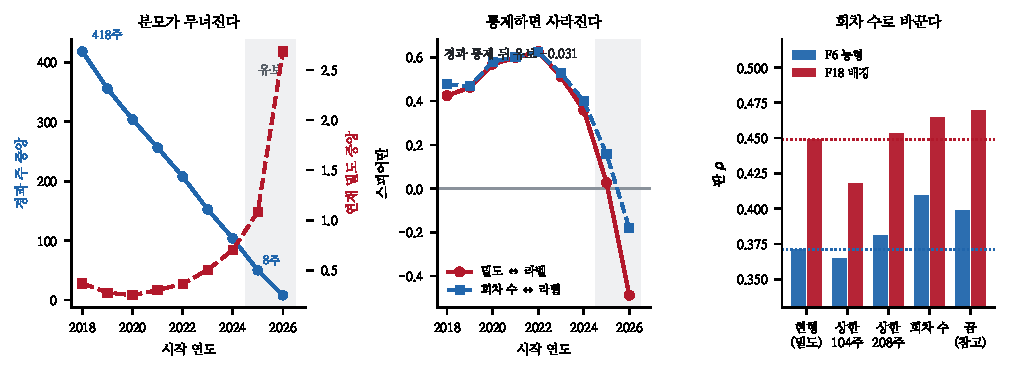
\includegraphics[width=\textwidth]{figs/denom.pdf}
\caption{왼쪽 --- 분모가 무너진다. 가운데 --- 통제하면 사라진다.
오른쪽 --- 회차 수로 바꾼다.}
\end{figure*}

\section{분모에 긁은 날이 박혀 있었다}

\begin{table}[t]
\centering\tsize
\caption{웹툰 시작 연도별. 긁은 날 2026-07-01 기준.}
\begin{tabular}{lrrrr}
\toprule
연 & n & 경과 주 & 밀도 & 완결율 \\
\midrule
2018 & 36 & \textbf{418} & 0.367 & 94.4\% \\
2021 & 382 & 256 & 0.302 & 86.6\% \\
2022 & 431 & 208 & 0.364 & 86.5\% \\
2024 & 450 & 104 & 0.703 & 59.3\% \\
2025 & 441 & 50 & 1.084 & 33.6\% \\
\textbf{2026} & 270 & \textbf{8} & \textbf{2.685} & \textbf{20.7\%} \\
\bottomrule
\end{tabular}
\end{table}

\claimx{\textbf{분모가 418주에서 8주로 무너진다.} 축은 ``회차 수 $\div$
경과 주''인데 그 ``지금''이 긁은 날로 고정돼 있다 --- 2026년에 시작한
작품은 여덟 주치로 나눈다.}{완결율도 94.4\%에서 20.7\%로 떨어진다 ---
\textbf{분자도 잘려 있다.} 아직 연재 중인 작품의 회차 수는 최종값이 아니다.}

\claimx{\textbf{그러니 이 축은 ``얼마나 최근에 시작했나''를 잰다.} 그리고
유보 분할이 정확히 시작일로 정의된다(2025년 전후) --- \textbf{축이 분할
변수를 담고 있다.}}{노트 141이 누수를 세 층으로 나눴는데(라벨 상관 · 출처
플랫폼 · 시점) 이건 넷째다 --- \textbf{자질이 분할 변수의 함수인 경우.}}

\section{통제하면 사라진다}

\begin{table}[t]
\centering\tsize
\caption{밀도 $\leftrightarrow$ 라벨. 경과 주를 통제하기 전후.}
\begin{tabular}{lrrr}
\toprule
& n & 원래 & 경과 통제 뒤 \\
\midrule
학습 ($<$2025) & 2{,}078 & $+$.378 & \textbf{$+$.562} \\
\textbf{유보 (2025$\sim$)} & 711 & \textbf{$-$.312} & \textbf{$-$.031} \\
\bottomrule
\end{tabular}
\end{table}

\claimx{\textbf{유보의 $-$0.312 가 $-$0.031 로 사라진다.} 부호 역전이
경과 주 하나로 다 설명된다.}{그리고 학습에서는 오히려 강해진다($+$0.378
$\to$ $+$0.562) --- \textbf{진짜 연재 밀도는 학습에서도 유보에서도 좋은
신호인데, 분모가 그것을 가리고 있었다.}}

\claimx{\textbf{스물다섯 노트가 이것을 ``시들기''로 다뤘다.} 노트 182가
부호 역전을 잡고 가드를 만들려다 문턱이 흔들려 실패했고, 노트 205가 ``열
하나가 도메인 하나를 죽인다''로, 노트 206이 ``뒤집히는 열이 하나뿐이라
규칙을 못 세운다''로 닫았다.}{\textbf{전부 맞는 관찰이었고 전부 잘못된
층에서 보고 있었다} --- 시간이 축과 라벨의 관계를 바꾼 것이 아니라
\emph{축의 정의}가 시간을 담고 있었다.}

\section{회차 수로 바꾼다}

\begin{table}[t]
\centering\tsize
\caption{웹툰 \texttt{goods\_scale} 을 바꾸면.}
\begin{tabular}{lrrr}
\toprule
& F6 & F21 & \textbf{F18} \\
\midrule
현행(밀도) & .3709 & .4094 & \textbf{.4490} \\
분모 104주 상한 & .3649 & .3803 & .4179 \\
분모 208주 상한 & .3812 & .3970 & .4532 \\
\textbf{회차 수} & \textbf{.4095} & .4224 & \textbf{.4643} \\
(끔 --- 참고) & .3990 & .4339 & .4694 \\
\bottomrule
\end{tabular}
\end{table}

\claimx{\textbf{회차 수가 제일 낫다}(F6 $+$0.039 · $t{=}5.2$). 분모에 상한을
두는 것은 오히려 나쁘다 --- 상한을 넘는 옛 작품과 안 넘는 새 작품이 서로
다른 자로 재게 된다.}{끄는 것과 견주면 F6 는 회차 수가 낫고 F18 · F21 은
끄는 쪽이 조금 낫다. \textbf{회차 수를 고른다} --- 자료를 버리는 것보다
고쳐 쓰는 것이 낫고, F6 의 차이가 제일 크다.}

\claimx{\textbf{만화도 같은 정의에 같은 붕괴다}(경과 주 569주 $\to$ 102주).
그런데 유보가 여섯 건뿐이라 판이 안 움직이고, 같이 고치면 F21 이 $-$0.001
이다 --- \textbf{웹툰만 고친다.}}{만화의 축이 틀린 것은 그대로다. 판이 안
움직인다는 것과 축이 옳다는 것은 다르다(노트 176 · 179).}

\section{이번엔 채택할 수 있다}

\claimx{\textbf{진단에 라벨을 한 칸도 안 썼다.} 경과 주가 418주에서 8주로
무너지는 것은 시작일과 긁은 날만 있으면 보인다.}{노트 206이 ``제일 큰 단일
개선인데 그 열을 유보 없이 고를 규칙이 안 선다''로 닫았는데 ---
\textbf{고를 필요가 없었다. 고치면 됐다.}}

\claimx{\texttt{lab/fixaxes.py} 로 넣어 자료를 읽을 때 고친다. 판이 F6
$+$0.4092 · F21 $+$0.4219 · \textbf{F18 $+$0.4614} 다 --- 챔피언이
$+$0.4490 에서 처음으로 옮겨 간다.}{\textbf{열한 번째 측정 아티팩트이고
처음으로 채택 가능한 것이다.} 앞의 열은 잡고 나면 판이 안 움직이거나
(노트 179 · 187 · 189 · 190) 고치는 규칙이 안 섰다(노트 206).}

\begin{table}[t]
\centering\tsize
\caption{남은 것.}
\begin{tabular}{ll}
\toprule
\textbf{같은 모양} & 다른 축에도 분모에 시간이 있나 \\
만화 & 축은 틀렸는데 판이 안 움직인다 \\
누수 넷째 층 & 자질이 분할 변수의 함수인 경우 \\
\bottomrule
\end{tabular}
\end{table}

첫 줄이 곧바로 할 수 있고 이 노트를 일반화한다. 웹툰 · 만화의 밀도는 축
파일의 \texttt{why} 에 ``258화/299주''라고 적혀 있어서 찾았다.
\textbf{다른 축에도 분모에 시간이 들어 있을 수 있다} --- 노트 164가 만든
\texttt{docs/AXIS\_MEANING.md} 를 열 도메인 $\times$ 다섯 축으로 훑으면서
``비율인가, 분모에 시간이 있나''만 보면 된다. \textbf{자료를 안 건드리고
문서만 읽어도 되는 검사이고, 이 흐름에서 제일 값싼 검사가 될 것이다.}

\end{document}
